\chapter{Hyperparameter optimisation of a classifying neural network}
\label{chp:simpleNN}

The basis of the adversarial neural network is formed by a common neural network trained on signal/background classification the output of which is then given to the adversary creating a negative backfeed for the training.

Before the adversarial, second network is added the classifying network is optimised on its own to make sure that its set-up is sufficient for the classification task.
During the adversarial training this set-up can be updated if the structure is not optimised for the additional task of a model independent of systematics.

This chapter describes the hyperparameter optimisation of the first network starting with the motivation  of the input information.
The second section explains the choice of the architecture followed by the step-wise set-up of the optimiser.
Lastly regularisation of the network is tested and described.
The overall aim of the description is to provide some understanding on the parameters available and their correlations and impact on the model to not only use these insights for the adversarial training but also to motivate possible problem solutions later on.


To train the network and to test its performance all the parts need to be in place. Therefore for all hyperparameters had to be initialized with values assumed to be around a good setup. Initially this was accomplished by starting with a very simple network using a miniml set of hyperparamters which were then worked up to a more and more optimised network. The results shown in this work are going to be based on the final choice of hyperparamters where only one paramter is then varied to explain the impact of the tuning. For that reason the first section will already introduce the final network structure which is then step by step to be motivated.

The structure was achieved within reason and the computational power constraints.


\section{Technical details}

\subsection{Machine learning libraries}

The artificial neural networks in this thesis were creates using the Keras python library.~\cite{chollet2015keras} 
Keras is an application programming interface written in python and able to run on Tensorflow, CNTK or Theano. It was developed by google and summarizes the necessary calculations for running a deep neural network training in fast and easy modules.
The backend is the package responsible for the underlying vector calculations needed for the network setup and training. In this work the tensorflow packag was used for backend.~\cite{tensorflow2015-whitepaper}

\subsection{Final setup of the network}

This subsection introduces the final setup of the classifying network


\section{The input variables}

got bdt variables

compared to simple kinematic

\begin{figure}
	\centering
	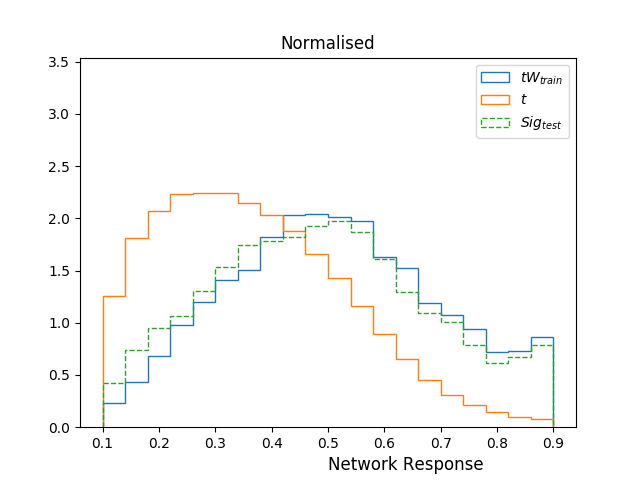
\includegraphics[width=\figwidth]{figures_simpleNN/test_simple.png}
\end{figure}



\section{The network architecture}

The architecture of the neural network is formed by its nodes and layers. The choice of the architecture is nontrivial and as a lot of aspect's of machine learning not an exact science.
However, one can make some assumptions about the appropriate architecture.
First of all the complexity of the model should about match the complexity of the task assigned. Although it usually is not trivial to find an estimator for a task's complexity and even less to match it to a certain architecture a test series often leads to a good estimate. Another possible thought is the amount of variables necessary to fully describe a system resulting in the minimum variable number necessary to input in the network which also gives a first estimate on how large the architecture should at least be.
Both the depth and the overall size of the model play a role. A simplified way of describing is by saying that the depth defines how often the input is processed during the network while the number of nodes is the number of features that can be kept during each step of processing.

In general an architecture that is too deep and wide will pick up too many features too fast and overtrains before it gets to a good minimum. This can be seen in an early divergence between the training loss and the validation loss. An architecture too simple is not able to pick up the features of the task at all and is not learning at all. The loss stays constant or changes very slowly.

In this work a testseries was performed, training a network for a wide range combinations of nodes and layers. For the sake of simplicity the number of nodes per layer was kept constant during each training. Two variables were then plotted against the size of the architecture. First the overall smallest loss the model achieved during the training was plotted. The other variable was the minimal difference between the training and the validation loss. To keep it simple the complexity of the architecture was defined as the product of nodes and layers. These are certainly not the most sophisticated indicators for the model's complexity and its performance. Nonetheless the plots show that region of good performance exists which was chosen for this analysis.

The good region lays between about x and y layers and x and y nodes each

\missingfigure{complexity}

\missingfigure{comparehighandlow}

Two different activation functions come to use in the neural network, the main function connects the nodes in the hidden layers while the last one converts the outputto a value between \num{0} and \num{1}. 

\missingfigure{elurelu}

Furthermore the activation function for the hidden layer is elu
the activation function 

\section{Setup of the optimisation}

For the most part of the optimisation SGD was used as the optimiser and its tuning is shown in this section in detail.
Adam was also tested out but not fully tuned due to constraints on tim and computational resources.

\subsection{Choice of the optimiser}

\subsection{Tuning the optimiser}



\section{Regularisation}